\documentclass[preprint,12pt,a4]{standalone}
\usepackage{geometry}   % my added package "geometry"
\geometry{letterpaper,tmargin=1in,bmargin=1in,lmargin=2.5cm,rmargin=2.5cm}
\usepackage{tikz}
\usetikzlibrary{calc,patterns,arrows.meta,shapes.arrows,intersections,positioning}
\usetikzlibrary{decorations.pathmorphing,backgrounds,fit,petri}
\usepackage{standalone}
%
\begin{document}
	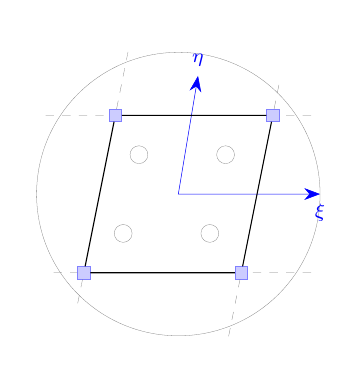
\begin{tikzpicture} [{place/.style={rectangle,draw=blue!50,fill=blue!20,ultra thin,inner sep=0.8mm}},{place2/.style={circle,draw=black!50,ultra thin,inner sep=0.8mm}},{linest/.style={color=gray,ultra thin}}]
		%%circle
		\draw [linest,fill=white](5.2,3.5) circle [radius=18mm];
		%axes
		\draw [{Stealth[length=2mm]}-{Stealth[length=2mm]}, help lines,blue] (7,3.5)node[below,font=\scriptsize]{$\xi$} -- (5.2,3.5) -- (5.45,5)node[above,font=\scriptsize] {$\eta$};
		%%element Nodes
		\node at (4.0,2.5) [place] (1) {};
		%\node at (5.0,2.5) [place] (2) {};
		\node at (6.0,2.5) [place] (3) {};
		%\node at (4.2,3.5) [place] (4) {};
		%\node at (5.2,3.5) [place] (5) {};
		%\node at (6.2,3.5) [place] (6) {};
		\node at (4.4,4.5) [place] (7) {};
		%\node at (5.4,4.5) [place] (8) {};
		\node at (6.4,4.5) [place] (9) {};
		
		\node at (4.5,3.0) [place2] {};
		\node at (5.6,3.0) [place2] {};
		\node at (4.7,4.0) [place2] {};
		\node at (5.8,4.0) [place2] {};
		\node at (3.5,2.5) [place2, draw = none] (10) {};
		\node at (7.0,2.5) [place2, draw = none] (11) {};
		\node at (3.4,4.5) [place2, draw = none] (12) {};
		\node at (7.0,4.5) [place2, draw = none] (13) {};
		\node at (3.9,2.0) [place2, draw = none] (14) {};
		\node at (5.8,1.5) [place2, draw = none] (15) {};
		\node at (4.6,5.5) [place2, draw = none] (16) {};
		\node at (6.5,5.0) [place2, draw = none] (17) {};
		%%element border
		\draw [-] (1) --(3)--(9)--(7)--(1);
		\draw [dashed,linest] (10) -- (1)--(14);
		\draw [dashed,linest] (11) -- (3)--(15);
		\draw [dashed,linest] (12) -- (7)--(16);
		\draw [dashed,linest] (13) -- (9)--(17);
	\end{tikzpicture}
\end{document}